% !TeX program = pdflatex
%==============================================================================
%  Aula 10 --- KNN e Árvores de Classificação
%  VERSÃO DO ALUNO: texto para leitura autônoma, fora da sala.
%  (O roteiro de sala é "10 KNN e Arvores de Classificacao.tex".)
%==============================================================================
\documentclass[11pt,a4paper]{article}
\usepackage[aluno]{../../recursos/latex/estilo-notas}
\usepackage{placeins} % \FloatBarrier: a Figura 1 não passa para a seção das árvores

\title{}
\date{}

\begin{document}
\cabecalhoaula{10}{KNN e Árvores de Classificação}{AME §8.3--8.6; ISLP §4.7.6 e cap.~8}

%==============================================================================
\section*{O que você vai aprender}
%==============================================================================
Ao final desta aula você deve ser capaz de:
\begin{itemize}[leftmargin=1.4cm]
  \item adaptar o KNN da regressão para classificação e reconhecê-lo como
        classificador \emph{plug-in};
  \item construir uma árvore de classificação, que prediz pela moda de cada folha;
  \item definir o índice de Gini e a entropia como medidas de impureza e explicar
        por que a taxa de erro não é usada para dividir os nós;
  \item usar \emph{bagging}, florestas aleatórias e \emph{boosting} em
        classificação;
  \item comparar os classificadores do curso e escolher entre eles segundo a
        estrutura dos dados e o objetivo da análise.
\end{itemize}

\noindent
Esta é a última aula sobre classificação. Os dois métodos que ela estuda, o KNN e as
árvores, já apareceram em regressão, nas Aulas~04 e~05, e quase tudo o que se faz aqui
é adaptá-los a uma resposta qualitativa: a média das respostas dá lugar à
\emph{moda}, e o erro quadrático médio dá lugar a uma medida de \emph{impureza}.

Fixemos a notação. A resposta $Y$ assume valores num conjunto finito $\mathcal{C}$ de
classes, e as observações de treino são $(\X_1,Y_1),\dots,(\X_n,Y_n)$, com
$\X_i\in\R^p$. Na Aula~07 vimos que, sob a perda 0--1, o classificador de menor risco
é o classificador de Bayes,
\[
  g^*(\x)=\argmax_{c\in\mathcal{C}}\ \Prob(Y=c\mid\X=\x),
\]
e que um classificador \emph{plug-in} substitui cada $\Prob(Y=c\mid\X=\x)$ por uma
estimativa $\widehat\Prob(Y=c\mid\x)$ e atribui $\x$ à classe de maior probabilidade
estimada. Os dois métodos desta aula são classificadores \emph{plug-in}.

%==============================================================================
\section{KNN para classificação}
%==============================================================================
Seja $d$ uma distância em $\R^p$, em geral a euclidiana. Como na Aula~04, para cada
$\x$ indicamos por $d^k_{\x}$ a distância de $\x$ à $k$-ésima observação de treino
mais próxima e por
\[
  \mathcal{N}_{\x}^{(k)}=\{i : d(\X_i,\x)\le d^k_{\x}\}
\]
o conjunto dos índices das $k$ observações de treino mais próximas de $\x$. Supomos
que não há empates entre as distâncias, de modo que esse conjunto tem exatamente $k$
elementos.

\begin{definicao}[KNN para classificação]
O classificador dos $k$ vizinhos mais próximos atribui a $\x$ a classe mais frequente
entre as respostas dos seus $k$ vizinhos:
\begin{equation}\label{eq:knncls}
  \ghat(\x) = \operatorname{moda}\{Y_i : i\in\mathcal{N}_{\x}^{(k)}\}.
\end{equation}
\end{definicao}

Em outras palavras, cada vizinho vota na sua classe, e vence a mais votada: é o
\emph{voto da maioria}. Se duas ou mais classes empatam no número de votos, a moda não
é única, e é preciso uma regra de desempate.

O KNN é um classificador \emph{plug-in}. Para cada classe $c$, estime
\[
  \widehat\Prob(Y=c\mid\x) = \frac{1}{k}\sum_{i\in\mathcal{N}_{\x}^{(k)}}\1{Y_i=c},
\]
a proporção de vizinhos de $\x$ que pertencem à classe $c$. Cada estimativa está em
$[0,1]$ e, como cada vizinho pertence a exatamente uma classe, as estimativas somam
$1$ sobre $\mathcal{C}$: formam uma distribuição de probabilidade sobre as classes.
Como $k\,\widehat\Prob(Y=c\mid\x)$ é o número de votos da classe $c$, a classe de maior
probabilidade estimada é a mais votada, isto é,
$\argmax_{c}\widehat\Prob(Y=c\mid\x)=\ghat(\x)$.

Essa estimativa mostra também em que sentido o KNN de classificação é uma adaptação
direta do de regressão. Como $\Prob(Y=c\mid\X=\x)=\E\big[\1{Y=c}\mid\X=\x\big]$, a
probabilidade condicional de cada classe é a função de regressão da variável
indicadora $\1{Y=c}$, e $\widehat\Prob(Y=c\mid\x)$ é exatamente o estimador KNN da
Aula~04 aplicado às respostas $\1{Y_1=c},\dots,\1{Y_n=c}$.

O número de vizinhos $k$ controla a flexibilidade do classificador. A
Figura~\ref{fig:knncls} mostra as fronteiras de decisão para $k=1$, $15$ e $120$. Com
$k=1$, e sem observações repetidas, cada observação de treino é a sua própria vizinha
mais próxima, já que $d(\X_i,\X_i)=0$; logo $\ghat(\X_i)=Y_i$ para todo $i$, e a
acurácia de treino é igual a $1$, qualquer que seja o desempenho do classificador em
observações novas.

\begin{figure}[htbp]
  \centering
  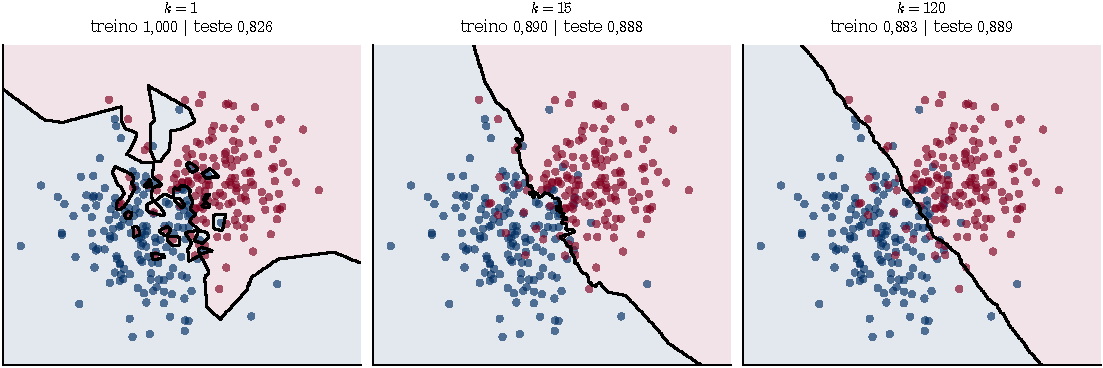
\includegraphics[width=\textwidth]{../../recursos/figuras/10-fronteiras-knn.pdf}
  \caption{Fronteiras de decisão do KNN com $n=300$ observações de treino; as
  acurácias de teste foram calculadas em $10\,000$ observações novas. Com $k=1$, a
  fronteira é muito recortada e forma ilhas em torno de observações isoladas; a
  acurácia de treino é exatamente $1{,}000$, e a de teste é a pior das três,
  $0{,}826$. Com $k=15$, a fronteira fica mais suave, e a acurácia de teste sobe para
  $0{,}888$; com $k=120$, a fronteira é quase uma reta, e a acurácia de teste
  praticamente não muda, $0{,}889$. Como na Figura~1 da Aula~04, é o $k$ pequeno que
  corresponde ao ajuste mais flexível.}
  \label{fig:knncls}
\end{figure}

\begin{atencao}
Valem os cuidados da Aula~04. Como o KNN se baseia numa distância, padronize as
covariáveis: na distância euclidiana, uma covariável medida numa escala maior domina
a soma dos quadrados das diferenças. E lembre da \emph{maldição da dimensionalidade}:
o KNN não seleciona covariáveis, e o seu desempenho piora quando há muitas
covariáveis irrelevantes, que entram na distância com o mesmo peso das relevantes. Em
problemas binários, use $k$ ímpar para evitar empates na votação.
\end{atencao}

\FloatBarrier

%==============================================================================
\section{Árvores de classificação}
%==============================================================================
As árvores de classificação são o análogo das árvores de regressão da Aula~05. Uma
árvore particiona o espaço das covariáveis, por divisões binárias sucessivas, em
regiões disjuntas $R_1,\dots,R_J$, as folhas. Para uma região $R$, sejam
$n_R=\#\{i:\X_i\in R\}$ o número de observações de treino em $R$ e
\[
  \widehat p_{R,c}=\frac{1}{n_R}\sum_{i:\X_i\in R}\1{Y_i=c},\qquad c\in\mathcal{C},
\]
a proporção da classe $c$ entre essas observações. A passagem da regressão para a
classificação exige duas adaptações: na predição de cada folha e no critério que
escolhe as divisões.

\subsection{Predição: a moda}
Numa folha $R_k$, a árvore prediz a classe majoritária, em vez da média das respostas:
\begin{equation}\label{eq:arvcls}
  \ghat(\x) = \operatorname{moda}\{Y_i : \X_i\in R_k\},\qquad \x\in R_k,
\end{equation}
e estima $\Prob(Y=c\mid\X=\x)$ por $\widehat p_{R_k,c}$, a proporção da classe $c$ na
folha. Pelo mesmo argumento usado no KNN, a classe majoritária é a de maior
$\widehat p_{R_k,c}$, e a árvore é também um classificador \emph{plug-in}.

É a substituição que o classificador de Bayes indica. Em regressão, sob a perda
quadrática, o alvo é a média condicional $\E[Y\mid\X=\x]$ (Aula~01), e a árvore o
estima pela média das respostas da folha. Em classificação, sob a perda 0--1, o alvo é
$g^*(\x)$, a moda da distribuição condicional de $Y$ dado $\X=\x$ (Aula~07), e a
árvore o estima pela moda das respostas da folha.

\subsection{Critério de divisão: impureza}\label{sec:impureza}
A segunda adaptação responde à pergunta:

\begin{center}\itshape
  como uma árvore decide a melhor pergunta a fazer em cada nó,\\
  quando o alvo é uma classe?
\end{center}

\noindent
Em regressão, a Aula~05 escolhia a divisão de menor EQM, mas o EQM não faz sentido
com $Y$ qualitativo. A medida \emph{óbvia}, a taxa de erro, é justamente a que não
funciona, e veremos por quê depois de definir as duas que funcionam.

Uma divisão é boa quando produz regiões \emph{puras}, isto é, regiões em que as
observações de treino são, idealmente, todas da mesma classe. Para medir o quanto uma
região $R$ se afasta disso, usam-se as medidas de impureza
\begin{align}
  \text{Índice de Gini:}\quad & G(R) = \sum_{c\in\mathcal{C}} \widehat p_{R,c}\,(1-\widehat p_{R,c}),
  \label{eq:gini}\\
  \text{Entropia:}\quad & D(R) = -\sum_{c\in\mathcal{C}} \widehat p_{R,c}\,\log_2 \widehat p_{R,c},
  \label{eq:entropia}
\end{align}
com a convenção $0\log_2 0=0$. A base do logaritmo só multiplica $D$ por uma constante
positiva e não altera nenhuma das comparações que faremos; a base~2 é a da
Figura~\ref{fig:impureza}. A terceira medida é a taxa de erro de classificação,
\[
  E(R)=1-\max_{c\in\mathcal{C}}\widehat p_{R,c},
\]
a proporção de observações de treino de $R$ que a classe majoritária classifica
errado.

\begin{proposicao}\label{prop:impureza}
As medidas $G(R)$ e $D(R)$ se anulam se e somente se $R$ é pura, isto é, se
$\widehat p_{R,c}=1$ para alguma classe $c$. Além disso,
$G(R)\le 1-1/\abs{\mathcal{C}}$ e $D(R)\le\log_2\abs{\mathcal{C}}$, com igualdade, nos
dois casos, se e somente se as classes estão equilibradas, isto é, se
$\widehat p_{R,c}=1/\abs{\mathcal{C}}$ para toda classe $c$.
\end{proposicao}
\begin{proof}
Como $0\le\widehat p_{R,c}\le1$, cada parcela $\widehat p_{R,c}(1-\widehat p_{R,c})$ e
cada parcela $-\widehat p_{R,c}\log_2\widehat p_{R,c}$ é não negativa, e se anula se e
somente se $\widehat p_{R,c}\in\{0,1\}$. Como as proporções somam $1$, estarem todas em
$\{0,1\}$ equivale a uma delas valer $1$, o que prova a primeira afirmação.

Para o máximo de $G$, note que
$G(R)=\sum_c\widehat p_{R,c}-\sum_c\widehat p_{R,c}^{\,2}=1-\sum_c\widehat p_{R,c}^{\,2}$.
Pela desigualdade de Cauchy--Schwarz,
\[
  1=\Big(\sum_{c\in\mathcal{C}}\widehat p_{R,c}\cdot 1\Big)^2
  \le\abs{\mathcal{C}}\sum_{c\in\mathcal{C}}\widehat p_{R,c}^{\,2},
\]
com igualdade se e somente se as proporções são todas iguais; logo
$G(R)\le1-1/\abs{\mathcal{C}}$, com igualdade exatamente nesse caso. Para o máximo de
$D$, seja $\mathcal{C}_+$ o conjunto das classes com $\widehat p_{R,c}>0$. Pela
desigualdade de Jensen aplicada à função côncava $\log_2$, com os pesos
$\widehat p_{R,c}$,
\[
  D(R)=\sum_{c\in\mathcal{C}_+}\widehat p_{R,c}\log_2\frac{1}{\widehat p_{R,c}}
  \le\log_2\sum_{c\in\mathcal{C}_+}\widehat p_{R,c}\,\frac{1}{\widehat p_{R,c}}
  =\log_2\abs{\mathcal{C}_+}\le\log_2\abs{\mathcal{C}} .
\]
Como $\log_2$ é estritamente côncava, a primeira desigualdade vale com igualdade se e
somente se $\widehat p_{R,c}$ é constante em $\mathcal{C}_+$, e a segunda, se e
somente se $\mathcal{C}_+=\mathcal{C}$; as duas juntas equivalem a
$\widehat p_{R,c}=1/\abs{\mathcal{C}}$ para toda classe $c$.
\end{proof}

Seja $I$ uma das medidas $G$ ou $D$. Quando uma região $R$, com $n_R$ observações de
treino, é dividida em $R_1=\{\x\in R: x_j<t\}$ e $R_2=\{\x\in R: x_j\ge t\}$, com
$n_1$ e $n_2$ observações ($n_1+n_2=n_R$), a impureza depois da divisão é a média das
impurezas das duas regiões ponderada pelo tamanho delas, e a redução de impureza é
\[
  \Delta I = I(R)-\Big[\frac{n_1}{n_R}\,I(R_1)+\frac{n_2}{n_R}\,I(R_2)\Big].
\]
A cada passo, escolhem-se a covariável $x_j$ e o corte $t$ que maximizam $\Delta I$.
Como $I(R)$ e $n_R$ não dependem da divisão, isso equivale a minimizar
$n_1I(R_1)+n_2I(R_2)$, o análogo da soma de quadrados minimizada na Aula~05: lá, a soma
de quadrados de $R_m$ é $n_m$ vezes o EQM de $R_m$, de modo que cada região também pesa
pelo seu número de observações.

\begin{figure}[htbp]
  \centering
  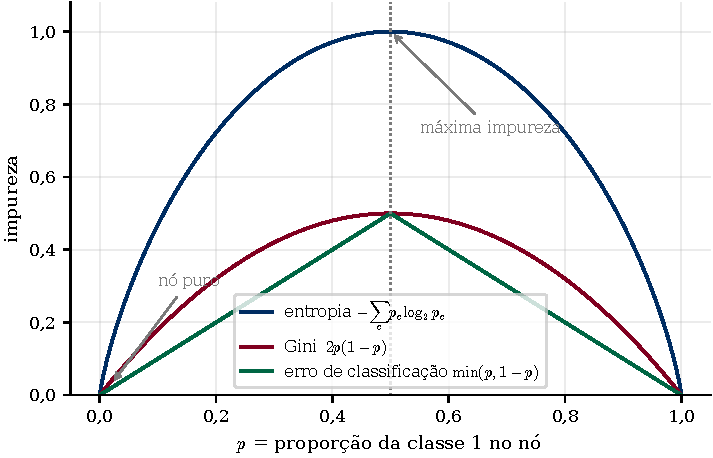
\includegraphics[width=0.62\textwidth]{../../recursos/figuras/10-impureza.pdf}
  \caption{As três medidas num nó com duas classes, em função da proporção $p$ da
  classe~1: o Gini é $2p(1-p)$, a entropia é $-p\log_2p-(1-p)\log_2(1-p)$ e o erro de
  classificação é $\min(p,1-p)$. As três se anulam nos extremos, onde o nó é puro, e
  são máximas em $p=1/2$. A diferença que importa está na forma: Gini e entropia são
  estritamente côncavas e suaves, enquanto o erro de classificação é formado por dois
  segmentos de reta, com um bico em $p=1/2$ e derivada constante de cada lado.}
  \label{fig:impureza}
\end{figure}

\begin{ideia}[Por que não usar a taxa de erro para dividir?]
No caso de duas classes, a taxa de erro de um nó com proporção $p$ da classe~1 é
$\min(p,1-p)$, a curva verde da Figura~\ref{fig:impureza}, que é linear em cada uma
das metades $[0,1/2]$ e $[1/2,1]$. Isso tem uma consequência séria. Considere um nó
com $400$ observações e $p=0{,}75$, e uma divisão que produza dois filhos de $200$
observações, um com $p=0{,}50$ e outro com $p=1{,}00$. O erro do pai é $0{,}25$, e o
erro ponderado dos filhos é $\tfrac12(0{,}50)+\tfrac12(0)=0{,}25$: a redução é zero,
embora um dos filhos seja puro, o que é claramente um progresso.

Não é uma coincidência do exemplo. Se um nó com $n$ observações e proporção $p$ é
dividido em filhos com $n_1$ e $n_2$ observações e proporções $p_1$ e $p_2$, então
$p=(n_1p_1+n_2p_2)/n$, porque as observações da classe~1 do nó são as dos dois filhos
somadas. Se a classe majoritária é a mesma nos dois filhos, $p_1$ e $p_2$ estão na
mesma metade de $[0,1]$, onde o erro é linear, e a média ponderada dos erros dos
filhos é o erro do pai: a redução é zero. Gini e entropia, por serem estritamente
côncavas, registram qualquer ganho de pureza: a média ponderada das impurezas dos
filhos é estritamente menor que a do pai sempre que $p_1\ne p_2$. No exemplo, o Gini
cai de $2(0{,}75)(0{,}25)=0{,}375$ para
$\tfrac12\cdot2(0{,}50)(0{,}50)+\tfrac12\cdot0=0{,}250$. A taxa de erro continua útil
na \emph{poda}, onde o que interessa é justamente o desempenho de classificação.
\end{ideia}

\begin{exemplo}[Escolha de divisão pelo Gini]
O [AME] considera dez hospitais e quer predizer se um hospital tem tomógrafo a partir
de duas covariáveis binárias: ter especialidade em cardiologia e ter mais de $100$
leitos. A tabela mostra, para cada uma das duas divisões possíveis da raiz, o número
de hospitais em cada região, quantos deles têm tomógrafo e o Gini
$2\widehat p(1-\widehat p)$ da região, com $\widehat p$ a proporção de hospitais com
tomógrafo.
\begin{center}\small
\renewcommand{\arraystretch}{1.3}
\begin{tabular}{@{}llccc@{}}
\toprule
divisão & região & hospitais & com tomógrafo & Gini \\
\midrule
cardiologia        & sim & $4$ & $2$ & $2\cdot\frac24\cdot\frac24=\frac12$ \\
                   & não & $6$ & $4$ & $2\cdot\frac46\cdot\frac26=\frac49$ \\
mais de 100 leitos & sim & $6$ & $5$ & $2\cdot\frac56\cdot\frac16=\frac5{18}$ \\
                   & não & $4$ & $1$ & $2\cdot\frac14\cdot\frac34=\frac38$ \\
\bottomrule
\end{tabular}
\end{center}
O Gini ponderado da divisão por cardiologia é
$\frac4{10}\cdot\frac12+\frac6{10}\cdot\frac49=\frac7{15}\approx0{,}467$, e o da
divisão por leitos é
$\frac6{10}\cdot\frac5{18}+\frac4{10}\cdot\frac38=\frac{19}{60}\approx0{,}317$. A
divisão por leitos deixa as regiões mais puras e é a escolhida. O [AME] chega a
$0{,}472$ e $0{,}326$ porque soma $\widehat p(1-\widehat p)$ nas duas regiões sem
ponderar pelo tamanho delas; a ordem entre as divisões, e portanto a escolha, é a
mesma.
\end{exemplo}

\begin{observacao}
Gini e entropia quase sempre escolhem as mesmas divisões. As duas curvas da
Figura~\ref{fig:impureza} têm quase a mesma forma: a menos de um fator de escala, que
não altera o $\argmin$, elas quase coincidem, e por isso o $\argmin$ sobre as
divisões candidatas raramente muda de uma medida para a outra. Não vale a pena,
portanto, incluir essa escolha numa busca por validação cruzada; é melhor gastar o
orçamento no $\alpha$ da poda ou na profundidade da árvore.
\end{observacao}

\noindent A construção segue as duas etapas da Aula~05: \emph{cresce-se} uma árvore
grande, dividindo as regiões pelo critério acima, e depois ela é \emph{podada} por
custo--complexidade, com $\alpha$ escolhido por validação cruzada. Valem também as
mesmas vantagens, que são a interpretabilidade, o tratamento direto de covariáveis
categóricas, a seleção automática de covariáveis e a captura de interações, e a mesma
desvantagem, os cortes perpendiculares aos eixos.

%==============================================================================
\section{\emph{Ensembles} para classificação}
%==============================================================================
As formas de agregar árvores também valem em classificação; o que muda é que cada
árvore agregada é agora uma árvore de classificação.
\begin{description}[leftmargin=2.6cm,style=nextline]
  \item[Bagging / Florestas] Ajustam-se $B$ árvores, cada uma numa amostra
        \emph{bootstrap} do treino, e as predições são agregadas pelo \emph{voto da
        maioria}. Pode-se também tomar a média das $B$ estimativas de
        $\Prob(Y=c\mid\x)$ e classificar pela maior; em geral isso é melhor, porque
        preserva a informação sobre a confiança de cada árvore, que o voto descarta.
        As florestas aleatórias diminuem a correlação entre as árvores sorteando, em
        cada nó, $m$ das $p$ covariáveis como candidatas à divisão; em classificação,
        a regra empírica é $m\approx\sqrt{p}$, mais agressiva que o $p/3$ usado em
        regressão. Aumentar $B$ não leva a superajuste, e o ajuste fornece, sem custo
        adicional, a estimativa do risco pelas observações deixadas fora de cada
        amostra \emph{bootstrap} (OOB, do inglês \emph{out-of-bag}) e medidas de
        importância das covariáveis.
  \item[Boosting] As árvores são ajustadas em sequência. A variante clássica em
        classificação é o AdaBoost: a cada rodada, as observações são reponderadas,
        com mais peso para as que estão sendo classificadas errado, e o classificador
        final é um voto ponderado dos aprendizes fracos, as árvores pequenas
        ajustadas em cada rodada. Um $B$ grande pode levar a superajuste, o que se
        evita com parada antecipada (\emph{early stopping}); o XGBoost é a
        implementação de referência.
\end{description}

\begin{observacao}
Codifique as classes por $y\in\{-1,+1\}$ e escreva o classificador final do AdaBoost
como o sinal de $f(\x)=\sum_{b=1}^{B}\alpha_b\,g_b(\x)$, em que $g_b(\x)\in\{-1,+1\}$
é a árvore ajustada na rodada $b$ e $\alpha_b>0$ é o seu peso no voto. Embora tenha
sido proposto por outro caminho (Freund e Schapire, 1995), o AdaBoost equivale a
construir $f$ por etapas, um termo de cada vez, minimizando a \emph{perda
exponencial} $e^{-y\,f(\x)}$ (Friedman, Hastie e Tibshirani, 2000). Essa perda
depende da observação apenas pelo produto $y\,f(\x)$, que é positivo quando a
classificação está certa, e cresce exponencialmente quando ele é negativo: um ponto
mal classificado por larga diferença pesa muito mais do que na perda 0--1, que vale
$1$ para qualquer erro. Isso explica a conhecida sensibilidade do AdaBoost a rótulos
errados.
\end{observacao}

%==============================================================================
\section{Comparando os classificadores do curso}
%==============================================================================
A tabela resume os classificadores vistos no curso.
\begin{center}\small
\renewcommand{\arraystretch}{1.3}
\begin{tabular}{@{}l>{\raggedright\arraybackslash}p{3.5cm}>{\raggedright\arraybackslash}p{3.2cm}>{\raggedright\arraybackslash}p{3.6cm}@{}}
\toprule
\textbf{Método} & \textbf{Fronteira} & \textbf{Interpretab.} & \textbf{Observações} \\
\midrule
Logística & linear (no \emph{log-odds}) & alta (coefs.) & dá probabilidades; robusta \\
LDA / QDA & linear / quadrática & média & ótimos sob gaussianidade \\
Bayes ingênuo & depende & média & forte com texto; descalibra se há correlação \\
KNN & muito flexível, local & baixa & sensível a escala e dimensão \\
Árvore & ``escada'' (eixos) & \textbf{altíssima} & instável sozinha \\
Florestas / Boosting & muito flexível & baixa & topo de desempenho em dados tabulares \\
SVM (kernel) & linear ou não linear & baixa & ótima com classes separadas \\
\bottomrule
\end{tabular}
\end{center}

\begin{ideia}
Nenhum método é melhor que os outros em todos os problemas; é o que se costuma
resumir na expressão ``não existe almoço grátis''. A escolha depende da estrutura dos
dados e do objetivo da análise, e quatro perguntas resolvem a maioria dos casos:
\begin{enumerate}[leftmargin=1.6cm,nosep]
  \item Preciso de probabilidades calibradas? Se sim, use a logística; se não,
        qualquer um serve (Aula~08).
  \item Preciso explicar a decisão a alguém? Se sim, use uma árvore ou a logística.
  \item Há muitas covariáveis irrelevantes? Então evite o KNN e a SVM com
        \emph{kernel} radial, que somam todas as coordenadas na distância, e prefira
        a logística com penalização Lasso, as florestas ou o \emph{boosting}.
  \item Os dados são tabulares e o objetivo é acertar? Comece pelo \emph{boosting}
        de árvores, que costuma ter o melhor desempenho, e use os outros como
        referência.
\end{enumerate}
Em qualquer caso, compare os candidatos por validação cruzada, com a métrica adequada
ao problema.
\end{ideia}

\begin{atencao}[o que a tabela não mostra: probabilidade não é escore]
A primeira das quatro perguntas, sobre probabilidades calibradas, parece uma
preferência de estilo, mas é uma restrição. A §7 da \texttt{Aula prática 10} compara
os sete métodos numa base em que a classe positiva é rara ($10\%$ das observações) e
mede duas coisas que vale guardar.

\emph{A acurácia deixa de distinguir os métodos.} Ela varia de $0{,}8989$ a
$0{,}9072$ entre os sete, uma faixa de menos de um ponto percentual, e quatro deles
empatam exatamente em $0{,}8989$, a acurácia de quem responde ``não'' para todos,
porque nunca preveem a classe positiva. Na mesma tabela, a precisão média (AP) varia
de $0{,}119$ a $0{,}453$, por um fator de quase quatro. Com uma classe rara, a
acurácia é dominada pela classe majoritária e não mede o que interessa.

\emph{O corte por custo pode não separar ninguém.} Para um falso negativo que custa
vinte falsos positivos, o corte ótimo da Aula~08 é
$c_{FP}/(c_{FP}+c_{FN})=1/21\approx0{,}0476$. Com ele, a árvore podada e o AdaBoost
mandam investigar todos os clientes, porque as probabilidades que eles produzem quase
nunca ficam abaixo de $0{,}05$. A cada mil clientes, entre os quais há $101$
positivos, a logística manda investigar $410$ e encontra $82$, e a SVM manda $493$ e
encontra $89$.

O corte $c_{FP}/(c_{FP}+c_{FN})$ é ótimo quando as probabilidades estimadas são
calibradas. Antes de usá-lo, confira a calibração do modelo (Aula~08) ou calibre-o, o
que é barato.
\end{atencao}

%==============================================================================
\section*{Resumo}
%==============================================================================
\begin{itemize}[leftmargin=1.4cm]
  \item KNN \eqref{eq:knncls}: voto da maioria entre os $k$ vizinhos; é
        \emph{plug-in}, com $\widehat\Prob(Y=c\mid\x)$ igual à proporção de vizinhos
        da classe $c$. Com $k=1$, a acurácia de treino é $100\%$, e a de teste é a
        pior das três da Figura~\ref{fig:knncls}.
  \item Árvore de classificação \eqref{eq:arvcls}: prediz a moda da folha e escolhe
        as divisões minimizando a impureza ponderada, medida pelo Gini
        \eqref{eq:gini} ou pela entropia \eqref{eq:entropia}.
  \item A taxa de erro não serve para dividir, porque é linear por partes e registra
        redução zero em divisões que aumentam a pureza
        (Figura~\ref{fig:impureza}); serve para podar.
  \item Os \emph{ensembles} valem em classificação: florestas com $m\approx\sqrt p$ e
        o AdaBoost, que equivale a \emph{boosting} com perda exponencial.
  \item Nenhum método é melhor em todos os problemas: escolha pela estrutura dos dados
        e pelo objetivo, e compare por validação cruzada com a métrica adequada
        (Aula~08).
\end{itemize}

\paragraph{Leitura recomendada.} [AME] §8.3 (árvores de classificação, com o exemplo
do tomógrafo usado aqui), §8.4 e §8.5 (\emph{bagging}, florestas e \emph{boosting} em
classificação) e §8.6 (KNN). [ISLP] §4.7.6 (KNN) e Capítulo~8, em especial o §8.1.2,
que trata das árvores de classificação e dos critérios de impureza.

\paragraph{Para praticar.} \texttt{Lista teorica 10.pdf} (teórica, com gabarito) e \texttt{Lista prática 10.ipynb} (prática, para completar as lacunas), nesta mesma pasta.

\end{document}
